\section{Motivation} \label{sec:moti}

In this section we use a simplified one-dimensional PNP model to illustrate the 
principal difficulties encountered in the numerical solution. Table~\ref{Table:used-constants} 
shows relevant constants. Fig.~\ref{fig:comsol-conc-volt} shows a typical solution for $C$ and $\phi$
at $t=0.1\ s$ and $t=3.0\ s$. 

\begin{table}[!ht]
\caption{Constants used in the Poisson-Nernst-Planck system of equations.}
\centering
\label{Table:used-constants}
{
\begin{tabular}{llll}
  \hline \hline
  Constant&Value&Unit&Description\\
  \hline
  $D$&$10\times10^{-11}$&$\frac{m^2}{s}$&Diffusion constant\\
  $z$&1&-&Charge number\\
  $F$&96,485&$\frac{C}{mol}$&Faraday number\\
  $R$&8.31&$\frac{J}{mol\cdot K}$&The gas constant\\
  $\mu\ \left( = \frac{D}{RT}\right)$&$4.11\times 10^{-14}$&$\frac{s}{mol\cdot K}$&Mobility\\
  $C_{0}$&1,200&$\frac{mol}{m^3}$&Anion concentration\\
  $\varepsilon$&0.025&$\frac{F}{m}$&Electric permittivity\\
  $l$&$200\times10^{-6}$&$m$& length scale\\
  \hline
  \hline
\end{tabular}
}
\end{table}

\noindent

\begin{figure}[!ht]
  \begin{centering}
      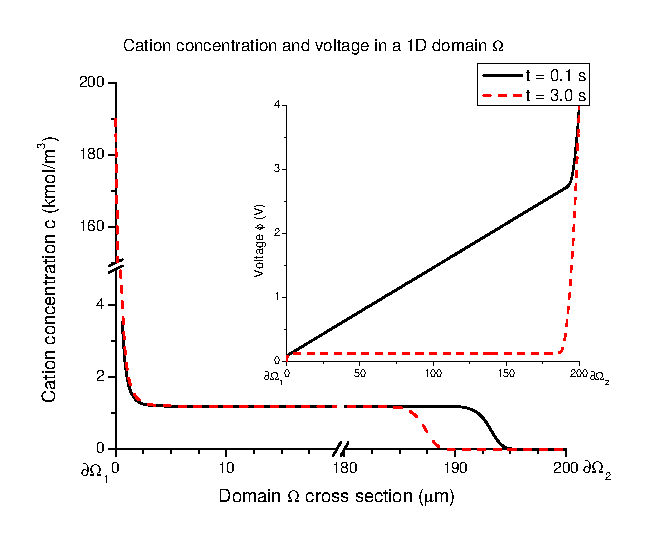
\includegraphics{comsol_conc_volt}
  \caption{Sample concentration $C$ and voltage $\phi$
           in a 1D domain $\Omega\subset\mathbb{R}$.
           Dirichlet boundary conditions ($V_{\partial \Omega_1}=0\ V$
           and $V_{\partial \Omega_2}=4\ V$) were
	   applied to the Poisson equation \eqref{eq:poisson} and Neumann conditions
	   to the Nernst-Planck equation \eqref{eq:nernst-planck}.}
\label{fig:comsol-conc-volt}
  \end{centering}
\end{figure}

The reader can observe that the solution has 
two notable characteristics: For the most part of the domain $\Omega$,
the gradient $\nabla C = 0$. Close to $\partial \Omega_2$, $\nabla C$ is
nonzero and moving in time, and $\nabla C$ is very large at $\partial \Omega_1$.
At the same time, $\phi$ is a "nice" smooth function for the most part of 
$\Omega$ but it has a large gradient at $\partial \Omega_2$.
This makes the choice of an optimal mesh highly problematic. Even if the 
solution was stationary, an optimal mesh for $C$ could never be 
optimal for $\phi$ and vice versa.

Furthermore, the shape of the solution in Fig.~\ref{fig:comsol-conc-volt}
suggests that the polynomial degree of finite elements in the middle
of the domain $\Omega$ and near the boundaries $\partial \Omega_1,\ \partial \Omega_2$
should be different --- large high-degree elements should be used in the middle of the 
domain while small low-degree ones should be used in the boundary layers.  
The qualitative differences in the solution components $C$ and $\phi$ 
also suggest that using different meshes would be beneficial. 



